
%====================================================================
\begin{frame}{1. Rappel : la FSMD, un algorithme câblé}
\begin{columns}[T]
\begin{column}{0.50\textwidth}
\centering
\begin{tikzpicture}[font=\scriptsize,>=Stealth]
  \node[st] (s0) at (0,1.5) {$S_0$};
  \node[st] (s1) at (2.2,1.5) {$S_1$};
  \node[st] (s2) at (4.4,2.7) {$S_2$};
  \node[st] (s3) at (4.4,0.3) {$S_3$};
  \draw[<-,thick] (s0.west) -- ++(-0.6,0) node[left,lab]{reset};
  \draw[->,thick] (s0) -- (s1);
  \draw[->,thick] (s1) to[bend left=20] node[above,sloped,lab]{$R_2\neq 0$} (s2);
  \draw[->,thick] (s2) to[bend left=20] (s1);
  \draw[->,thick] (s1) -- node[below,sloped,lab]{$R_2=0$} (s3);
  \path[->,thick] (s3) edge[loop right] (s3);
\end{tikzpicture}

\vspace{2mm}
\footnotesize Calcul de $Y = A \times B$ par additions successives (registres $R_1,R_2,R_3$).
\end{column}
\begin{column}{0.50\textwidth}
\scriptsize
\renewcommand{\arraystretch}{1.3}
\begin{tabular}{|c|l|}
\hline
\rowcolor{\cS} $S_0$ & $R_1 \aff A$ ;\; $R_2 \aff B$ ;\; $R_3 \aff 0$ \\ \hline
\rowcolor{\cT} $S_1$ & si $R_2 = 0$ alors $S_3$ sinon $S_2$ \\ \hline
\rowcolor{\cU} $S_2$ & $R_3 \aff R_3 + R_1$ ;\; $R_2 \aff R_2 - 1$ ;\; $\to S_1$ \\ \hline
\rowcolor{\cV} $S_3$ & $Y \aff R_3$ ;\; fin \\ \hline
\end{tabular}
\end{column}
\end{columns}

\vspace{3mm}
\begin{block}{Ce qu'il faut remarquer}
\footnotesize
\begin{itemize}\setlength{\itemsep}{1pt}
 \item Le \alert{séquencement} (graphe d'états) \emph{est} l'algorithme : changer d'algorithme $=$ refaire la FSM.
 \item Les registres $R_i$ sont \alert{nommés} dans les actions et \alert{câblés} à l'UAL.
 \item Une action d'état peut faire \alert{plusieurs transferts en parallèle} ($S_2$).
\end{itemize}
\end{block}
\end{frame}

%====================================================================
\begin{frame}{2. L'idée : extraire le programme de la FSM}
  \begin{center}
    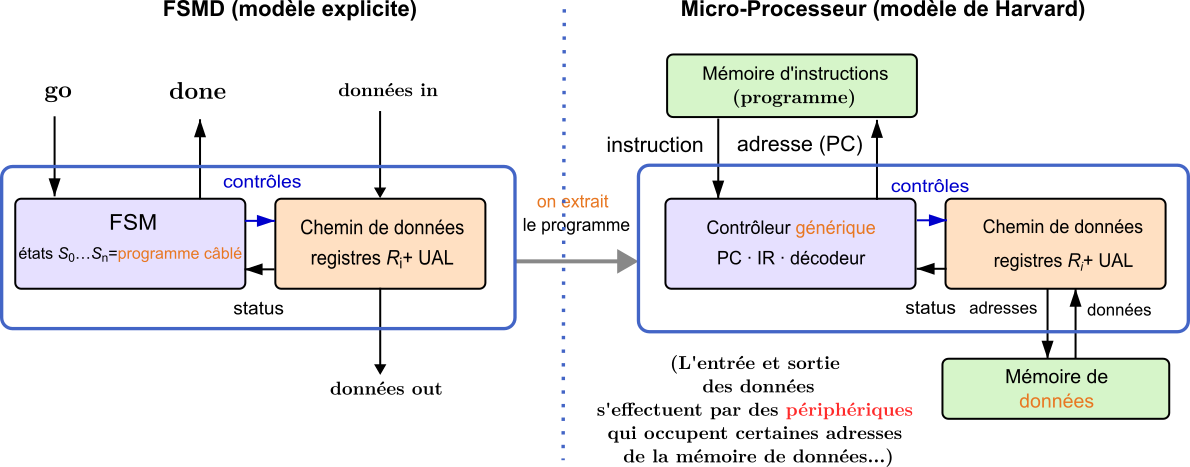
\includegraphics[scale=0.4]{./images/fsmd_proc.png}
  \end{center}

  \vspace{2mm}
  \begin{block}{Idée directrice}
  \footnotesize
  Si le séquencement est \emph{lu} dans une mémoire au lieu d'être câblé, la FSM devient générique (la même pour tout programme) :
  on obtient un \alert{processeur}. Le programme devient une \alert{donnée}.
  \end{block}
\end{frame}

%====================================================================
\begin{frame}{3. La mémoire de données et registres de travail}
  \begin{columns}[T]
    \begin{column}{0.44\textwidth}
      \footnotesize
      \textbf{Dans la FSMD} : quelques registres $R_i$, câblés à l'UAL, désignés \emph{par leur nom} dans les actions d'état.

      \medskip
      \textbf{Limite} : le nombre de registres est petit (coût en surface, en multiplexeurs).

      \medskip
      \textbf{Extension naturelle} :
      \begin{itemize}\setlength{\itemsep}{1pt}
        \item un \alert{banc de registres} : registres désignés par un \emph{numéro} (champ de l'instruction) ;
        \item une \alert{mémoire de données} : beaucoup de mots, désignés par une \emph{adresse}, mais \alert{non reliée directement à l'UAL}.
      \end{itemize}

      \medskip
      Deux instructions de transfert suffisent : \texttt{LD} (mémoire $\to$ registre) et \texttt{ST} (registre $\to$ mémoire).
    \end{column}

    \begin{column}{0.56\textwidth}
      \centering
      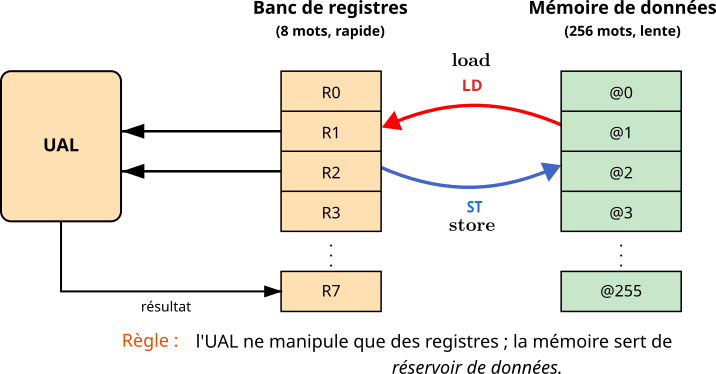
\includegraphics[scale=0.4]{./images/reg_mem.png}
    \end{column}
  \end{columns}

  \begin{block}{A retenir}
  \footnotesize
  On parle d'\textit{"architecture \texttt{load-store}""}
  \end{block}
\end{frame}

%====================================================================
\begin{frame}{4. Architecture de Harvard : deux mémoires, un contrôleur générique}
\centering
\begin{tikzpicture}[font=\scriptsize]
  \node[box,ctrl,minimum width=1.2cm] (pc) at (0,0) {PC};
  \node[box,mem,minimum width=2.6cm] (im) at (3.4,0) {Mémoire\\d'instructions};
  \node[box,ctrl,minimum width=2.8cm] (id) at (7.4,0) {IR + décodeur\\(unité de contrôle)};
  \draw[dat] (pc) -- (im) node[midway,above,lab]{adresse};
  \draw[dat] (im) -- (id) node[midway,above,lab]{instruction};
  \draw[dat,dashed] (id.north) -- ++(0,0.6) -| (pc.north) node[pos=0.25,above,lab]{PC $\leftarrow$ PC+1, ou saut};

  \node[box,data,minimum width=2.2cm] (rf) at (2.4,-2.7) {Banc de\\registres};
  \node[box,data,minimum width=1.6cm] (alu) at (6.0,-2.7) {UAL};
  \node[box,mem,minimum width=2.4cm] (dm) at (9.6,-2.7) {Mémoire\\de données};

  \draw[cmd] (id.south) to[out=-90,in=90] (rf.north);
  \draw[cmd] (id.south) to[out=-90,in=90] (alu.north);
  \draw[cmd] (id.south) to[out=-90,in=90] node[pos=0.55,right,lab]{commandes} (dm.north);

  \draw[dat] (rf.east) -- (alu.west) node[midway,above,lab]{opérandes};
  \draw[dat] (alu.east) -- (dm.west) node[midway,above,lab]{adresse};
  \draw[dat] (alu.south) -- ++(0,-0.6) -| ([xshift=3mm]rf.south) node[pos=0.25,below,lab]{résultat};
  \draw[dat] (dm.south) -- ++(-0cm,-1.0) -| ([xshift=-3mm]rf.south) node[pos=0.25,below,lab]{LD : donnée lue};

  \node[align=left,text width=3cm,font=\footnotesize] at (11.8,0.2)
    {\alert{Harvard} : deux mémoires, deux bus $\Rightarrow$ lecture de l'instruction et accès aux données \alert{simultanés}.};
\end{tikzpicture}

\vspace{1mm}
\footnotesize
\begin{tabular}{@{}ll@{}}
\textbf{FSMD} $\to$ \textbf{processeur} : & registres $\to$ banc de registres $+$ mémoire de données ; \\
& FSM spécifique $\to$ PC $+$ IR $+$ décodeur $+$ mémoire d'instructions.
\end{tabular}
\end{frame}

%====================================================================
\begin{frame}{5. Format d'une instruction : opcode, sources, destination}
  \begin{columns}[T]
    \begin{column}{0.64\textwidth}
      \centering
      \begin{tikzpicture}[font=\scriptsize]
        \node[anchor=west,font=\scriptsize\bfseries] at (0,2.0) {Format R (registre)};
        \node[field,fill=red!20, minimum width=1.68cm,anchor=west] at (0,1.05) {opcode};
        \node[field,fill=orange!25,minimum width=1.26cm,anchor=west] at (1.68,1.05) {rd};
        \node[field,fill=blue!15, minimum width=1.26cm,anchor=west] at (2.94,1.05) {rs1};
        \node[field,fill=blue!15, minimum width=1.26cm,anchor=west] at (4.20,1.05) {rs2};
        \node[field,fill=gray!15, minimum width=1.26cm,anchor=west] at (5.46,1.05) {--};
        \node[lab,anchor=south] at (0.84,1.45) {4 bits};
        \foreach \x in {2.31,3.57,4.83,6.09} {
          \node[lab,anchor=south] at (\x,1.45) {3};
        }
        \node[lab,anchor=north] at (0.84,0.65) {\texttt{0000}};
        \node[lab,anchor=north] at (2.31,0.65) {\texttt{011}};
        \node[lab,anchor=north] at (3.57,0.65) {\texttt{011}};
        \node[lab,anchor=north] at (4.83,0.65) {\texttt{001}};
        \node[lab,anchor=north] at (6.09,0.65) {\texttt{000}};
        \node[lab,anchor=west] at (6.8,1.05) {\texttt{ADD R3,R3,R1}};

        \node[anchor=west,font=\scriptsize\bfseries] at (0,-0.25) {Format I (immédiat / mémoire / saut)};
        \node[field,fill=red!20, minimum width=1.68cm,anchor=west] at (0,-0.8) {opcode};
        \node[field,fill=orange!25,minimum width=1.26cm,anchor=west] at (1.68,-0.8) {rd};
        \node[field,fill=blue!15, minimum width=1.26cm,anchor=west] at (2.94,-0.8) {rs1};
        \node[field,fill=green!20, minimum width=2.52cm,anchor=west] at (4.20,-0.8) {imm (6 bits)};
        \node[lab,anchor=north] at (0.84,-1.2) {\texttt{0100}};
        \node[lab,anchor=north] at (2.31,-1.2) {\texttt{001}};
        \node[lab,anchor=north] at (3.57,-1.2) {\texttt{000}};
        \node[lab,anchor=north] at (5.46,-1.2) {\texttt{000000}};
        \node[lab,anchor=west] at (6.8,-0.8) {\texttt{LD R1,[R0+0]}};
      \end{tikzpicture}
    \end{column}
    \begin{column}{0.36\textwidth}
      \scriptsize
      \begin{itemize}\setlength{\itemsep}{2pt}
       \item \colorbox{red!20}{opcode} : \emph{quelle} opération $\to$ décodeur $\to$ commandes ;
       \item \colorbox{blue!15}{rs1, rs2} : numéros des registres \emph{sources} ;
       \item \colorbox{orange!25}{rd} : registre \emph{destination} ;
       \item \colorbox{green!20}{imm} : constante, déplacement ou offset de saut.
      \end{itemize}
    \end{column}
  \end{columns}

  \vspace{2mm}

  \begin{block}{Mot de 16 bits}
    \footnotesize
    \texttt{ADD R3,R3,R1} $=$ \texttt{0000 0110 1100 1000} $=$ \texttt{0x06C8} \qquad
    \texttt{LD R1,[R0+0]} $=$ \texttt{0100 0010 0000 0000} $=$ \texttt{0x4200}

    \smallskip
    Une instruction n'est \alert{qu'un mot} stocké dans la mémoire d'instructions : le \og programme \fg{} est une liste de mots.
  \end{block}
\end{frame}

%====================================================================
\begin{frame}{6. Un jeu d'instructions minimal}
  \centering\footnotesize
  \renewcommand{\arraystretch}{1.25}
  \setlength{\tabcolsep}{5pt}
  \begin{tabular}{|l|l|c|c|l|}
    \hline
    \textbf{Classe} & \textbf{Instruction} & \textbf{Format} & \textbf{opcode} & \textbf{Effet (transfert de registres)} \\ \hline
    \rowcolor{\cU} Arithmétique & \texttt{ADD rd, rs1, rs2} & R & \texttt{0000} & $\R{rd} \aff \R{rs1} + \R{rs2}$ ;\; PC $\aff$ PC+1 \\
    \rowcolor{\cU} & \texttt{SUB rd, rs1, rs2} & R & \texttt{0001} & $\R{rd} \aff \R{rs1} - \R{rs2}$ ;\; PC $\aff$ PC+1 \\
    \rowcolor{\cU} & \texttt{ADDI rd, rs1, imm} & I & \texttt{0010} & $\R{rd} \aff \R{rs1} + \mathit{imm}$ ;\; PC $\aff$ PC+1 \\ \hline
    \rowcolor{\cS} Mémoire & \texttt{LD rd, [rs1+imm]} & I & \texttt{0100} & $\R{rd} \aff \M{\R{rs1}+\mathit{imm}}$ \\
    \rowcolor{\cS} & \texttt{ST rd, [rs1+imm]} & I & \texttt{0101} & $\M{\R{rs1}+\mathit{imm}} \aff \R{rd}$ \quad {\scriptsize(\emph{rd} lu comme source)} \\ \hline
    \rowcolor{\cT} Contrôle & \texttt{BEQ rd, rs1, imm} & I & \texttt{1000} & si $\R{rd}=\R{rs1}$ alors PC $\aff$ PC+$\mathit{imm}$ sinon PC+1 \\
    \rowcolor{\cT} & \texttt{JMP imm} & I & \texttt{1100} & PC $\aff$ $\mathit{imm}$ \\ \hline
  \end{tabular}

  \vspace{4mm}
  \begin{minipage}{0.9\textwidth}
    \footnotesize
    \begin{itemize}\setlength{\itemsep}{2pt}
       \item \texttt{R0} est câblé à $0$ : \texttt{ADDI R3,R0,0} met $R_3$ à zéro, \texttt{[R0+k]} désigne l'adresse absolue $k$.
       \item Une instruction $=$ \alert{un seul transfert} (la FSMD pouvait en faire plusieurs par état).
       \item \texttt{BEQ}/\texttt{JMP} sont les seules à modifier PC autrement que par $+1$ : ce sont les \alert{transitions} de la FSM.
    \end{itemize}
  \end{minipage}
\end{frame}

%====================================================================
\begin{frame}{7. Décodage : du mot binaire au pilotage du datapath}
  \centering
  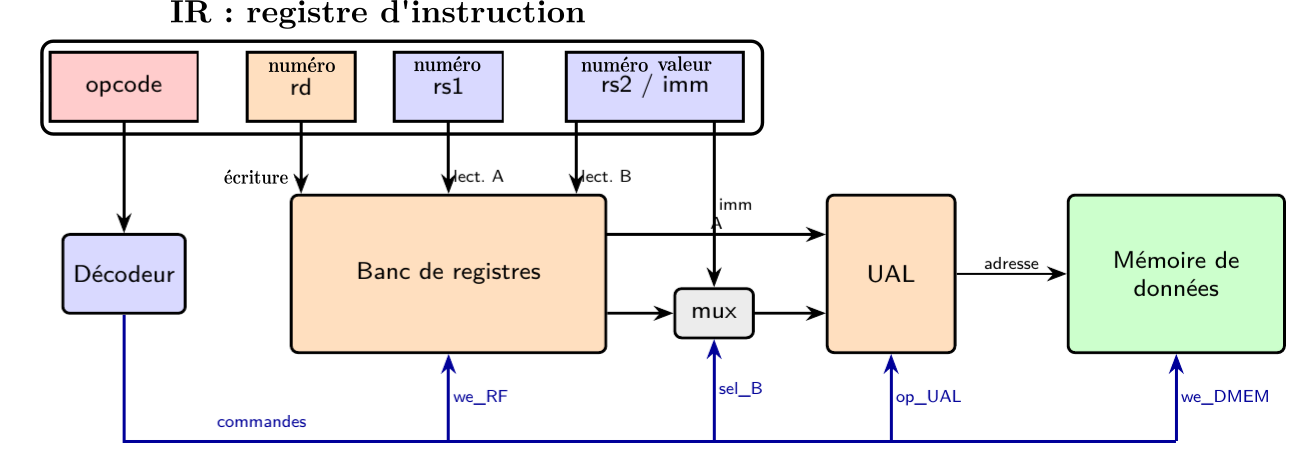
\includegraphics[scale=0.4]{./images/decodage_ir.png}
  \vspace{2mm}

  \begin{block}{Deux exemples}
    \footnotesize
    \texttt{ADD} : op\_UAL$=+$, sel\_B$=$rs2, we\_RF$=1$, we\_DMEM$=0$ \hfill
    \texttt{ST} : op\_UAL$=+$ (adresse), sel\_B$=$imm, we\_RF$=0$, we\_DMEM$=1$

    \smallskip
    Le décodeur est un circuit \alert{combinatoire} : opcode $\to$ commandes. Les numéros de registres vont \alert{directement} au banc de registres.
  \end{block}
\end{frame}

%====================================================================
\begin{frame}{8. Le cycle d'instruction : une FSM générique à la place de la FSM dédiée}
\begin{columns}[T]
  \begin{column}{0.50\textwidth}
  \centering
  \begin{tikzpicture}[font=\scriptsize,
    st/.style={circle,draw,thick,fill=blue!15,minimum size=1.5cm,align=center,inner sep=1pt}]
    \node[st] (f) at (0,0) {FETCH};
    \node[st] (d) at (2.5,0) {DECODE};
    \node[st] (e) at (5.0,0) {EXECUTE};
    \draw[dat] (f) -- (d);
    \draw[dat] (d) -- (e);
    \draw[dat] (e.south) -- ++(0,-0.5) -| (f.south);
    \node[align=center,text width=2.2cm,font=\tiny] at (0,-2.1) {IR $\aff$ IMEM[PC]\\PC $\aff$ PC+1};
    \node[align=center,text width=2.2cm,font=\tiny] at (2.5,-2.1) {lecture de rs1, rs2\\dans le banc de registres};
    \node[align=center,text width=2.4cm,font=\tiny] at (5.0,-2.1) {UAL / accès DMEM\\écriture dans rd ou PC};
  \end{tikzpicture}

  \vspace{1mm}
  \footnotesize
  Cette FSM est \alert{la même quel que soit le programme} : seul le contenu de la mémoire d'instructions change.
  \end{column}

  \begin{column}{0.45\textwidth}
    \scriptsize
    \renewcommand{\arraystretch}{1.2}
    \setlength{\tabcolsep}{3pt}
    \begin{tabular}{|p{2.5cm}|p{3.2cm}|}
    \hline
    \textbf{FSMD} & \textbf{Processeur} \\ \hline
    état $S_i$ & instruction à l'adresse PC $=i$ \\ \hline
    action $R_a \aff R_b \circ R_c$ & champs \texttt{opcode, rd, rs1, rs2} \\ \hline
    signaux de commande (câblés) & sorties du décodeur \\ \hline
    transition conditionnelle & \texttt{BEQ}, \texttt{JMP} (modifient PC) \\ \hline
    registres de travail & banc de registres $+$ mémoire de données \\ \hline
    \end{tabular}
    \end{column}
\end{columns}

\vspace{2mm}
\begin{block}{À retenir}
\footnotesize
Un processeur est une FSMD dont le \alert{séquencement est lu} en mémoire : \alert{un état $=$ une instruction}, \alert{PC $=$ registre d'état}.
\end{block}
\end{frame}

%====================================================================
\begin{frame}{9. Fil rouge : FSMD puis en programme}
\begin{columns}[T]
\begin{column}{0.44\textwidth}
\centering\footnotesize\textbf{FSMD}\par\vspace{1mm}
\scriptsize
\renewcommand{\arraystretch}{1.5}
\begin{tabular}{|c|l|}
\hline
\rowcolor{\cS} $S_0$ & $R_1 \aff A$ ;\; $R_2 \aff B$ ;\; $R_3 \aff 0$ \\ \hline
\rowcolor{\cT} $S_1$ & si $R_2 = 0$ alors $S_3$ sinon $S_2$ \\ \hline
\rowcolor{\cU} $S_2$ & $R_3 \aff R_3 + R_1$ ;\; $R_2 \aff R_2 - 1$ \\ \hline
\rowcolor{\cV} $S_3$ & $Y \aff R_3$ ;\; fin \\ \hline
\end{tabular}
\end{column}
\begin{column}{0.56\textwidth}
\centering\footnotesize\textbf{Programme} (mémoire d'instructions)\par\vspace{1mm}
\scriptsize
\renewcommand{\arraystretch}{1.1}
\begin{tabular}{|c|l|l|}
\hline
\textbf{PC} & \textbf{Instruction} & \textbf{Commentaire} \\ \hline
\rowcolor{\cS} 0 & \texttt{LD R1,[R0+0]} & $R_1 \aff A$ \\
\rowcolor{\cS} 1 & \texttt{LD R2,[R0+1]} & $R_2 \aff B$ \\
\rowcolor{\cS} 2 & \texttt{ADDI R3,R0,0} & $R_3 \aff 0$ \\ \hline
\rowcolor{\cT} 3 & \texttt{BEQ R2,R0,+4} & si $R_2=0$ aller en 7 \\ \hline
\rowcolor{\cU} 4 & \texttt{ADD R3,R3,R1} & $R_3 \aff R_3+R_1$ \\
\rowcolor{\cU} 5 & \texttt{ADDI R2,R2,-1} & $R_2 \aff R_2-1$ \\
\rowcolor{\cU} 6 & \texttt{JMP 3} & retour au test \\ \hline
\rowcolor{\cV} 7 & \texttt{ST R3,[R0+2]} & $Y \aff R_3$ \\
\rowcolor{\cV} 8 & \texttt{JMP 8} & boucle (fin) \\ \hline
\end{tabular}
\end{column}
\end{columns}

\vspace{2mm}
\begin{block}{Ce qui change}
\footnotesize
\begin{itemize}\setlength{\itemsep}{1pt}
 \item Entrées/sortie $A$, $B$, $Y$ : ce sont maintenant des \alert{cases de la mémoire de données} (@0, @1, @2).
 \item Un état à deux transferts ($S_2$) devient \alert{plusieurs instructions} : un transfert par instruction.
 \item Le graphe d'états a disparu : il est \alert{encodé dans les adresses et les sauts}.
\end{itemize}
\end{block}
\end{frame}

%====================================================================
\begin{frame}{10. Trace d'exécution pour $A=3$, $B=2$}
\centering
\scriptsize
\renewcommand{\arraystretch}{1.12}
\setlength{\tabcolsep}{5pt}
\begin{tabular}{|c|c|l|c|c|c|c|l|}
\hline
\textbf{n} & \textbf{PC} & \textbf{Instruction} & $R_1$ & $R_2$ & $R_3$ & $\M{2}$ & \textbf{Remarque} \\ \hline
1 & 0 & \texttt{LD R1,[R0+0]} & 3 & -- & -- & -- & \\
2 & 1 & \texttt{LD R2,[R0+1]} & 3 & 2 & -- & -- & \\
3 & 2 & \texttt{ADDI R3,R0,0} & 3 & 2 & 0 & -- & \\
\rowcolor{\cT} 4 & 3 & \texttt{BEQ R2,R0,+4} & 3 & 2 & 0 & -- & non pris : PC $\aff$ 4 \\
5 & 4 & \texttt{ADD R3,R3,R1} & 3 & 2 & 3 & -- & \\
6 & 5 & \texttt{ADDI R2,R2,-1} & 3 & 1 & 3 & -- & \\
7 & 6 & \texttt{JMP 3} & 3 & 1 & 3 & -- & PC $\aff$ 3 \\
\rowcolor{\cT} 8 & 3 & \texttt{BEQ R2,R0,+4} & 3 & 1 & 3 & -- & non pris \\
9 & 4 & \texttt{ADD R3,R3,R1} & 3 & 1 & 6 & -- & \\
10 & 5 & \texttt{ADDI R2,R2,-1} & 3 & 0 & 6 & -- & \\
11 & 6 & \texttt{JMP 3} & 3 & 0 & 6 & -- & \\
\rowcolor{\cT} 12 & 3 & \texttt{BEQ R2,R0,+4} & 3 & 0 & 6 & -- & \alert{pris} : PC $\aff$ 3+4 $=7$ \\
\rowcolor{\cV} 13 & 7 & \texttt{ST R3,[R0+2]} & 3 & 0 & 6 & \alert{6} & $Y = 6$ \\ \hline
\end{tabular}

\vspace{2mm}
\footnotesize
La FSMD fait la même chose en $1 + 2\times 2 + 1 + 1 = 7$ cycles ($S_0$, deux tours $S_1S_2$, $S_1$, $S_3$) ; le processeur exécute ici \alert{13 instructions} : on a échangé du \emph{temps} contre de la \emph{généralité}.
\end{frame}

%====================================================================
\begin{frame}{11. Bilan et ouverture}
\begin{columns}[T]
\begin{column}{0.5\textwidth}
\centering
\begin{tikzpicture}[font=\scriptsize]
  \node[font=\footnotesize\bfseries] at (1.8,2.4) {Harvard};
  \node[box,ctrl] (c) at (1.8,1.2) {CPU};
  \node[box,mem] (i) at (0,0) {IMEM};
  \node[box,mem] (d) at (3.6,0) {DMEM};
  \draw[dat,<->] (c) -- (i) node[midway,left,lab]{bus 1};
  \draw[dat,<->] (c) -- (d) node[midway,right,lab]{bus 2};
\end{tikzpicture}
\hspace{3mm}
\begin{tikzpicture}[font=\scriptsize]
  \node[font=\footnotesize\bfseries] at (1.0,2.4) {von Neumann};
  \node[box,ctrl] (c) at (1.0,1.2) {CPU};
  \node[box,mem,minimum width=2.2cm] (m) at (1.0,0) {MEM\\(instr. + données)};
  \draw[dat,<->] (c) -- (m) node[midway,right,lab]{bus unique};
\end{tikzpicture}
\end{column}
\begin{column}{0.5\textwidth}
\footnotesize
\textbf{Ce qu'on a ajouté} à la FSMD :
\begin{itemize}\setlength{\itemsep}{1pt}
 \item PC, mémoire d'instructions, IR, décodeur ;
 \item mémoire de données, \texttt{LD}/\texttt{ST}.
\end{itemize}
\textbf{Ce qu'on a gardé} : le chemin de données (registres + UAL) et l'idée « un état $=$ des transferts ».
\end{column}
\end{columns}

\vspace{3mm}
\begin{block}{Pour aller plus loin}
\footnotesize
\begin{itemize}\setlength{\itemsep}{2pt}
 \item \alert{von Neumann} : une seule mémoire pour code et données (plus souple, mais fetch et accès données se disputent le bus).
 \item \alert{Pipeline} : chevaucher fetch, decode et execute pour approcher une instruction par cycle.
 \item Jeux d'instructions plus riches : \texttt{CALL}/\texttt{RET}, pile, interruptions, entrées/sorties.
\end{itemize}
\end{block}
\end{frame}
